\documentclass{note}
\usepackage[python,table,pseudo]{mypackage}
\usepackage{xcolor}
\hypersetup{colorlinks=false,urlbordercolor=red}
\usepackage{footnote}
\makesavenoteenv{tabular}

\usepackage{tcolorbox}
% \begin{tcolorbox}[sharp corners, colback=green!30, colframe=green!80!blue, title=Another paragraph with title]

\renewcommand{\thefootnote}{\fnsymbol{footnote}}
\newcommand{\newterm}[1]{\textcolor{black}{\emph{\textbf{#1}}}}
\def\diag{\mathrm{diag}}

\title{深度学习笔记}
\author{陈鸿峥}
\date{{\builddatemonth\today}\protect\footnote{\text{Build \builddate\today}}} % protect!

\setcounter{secnumdepth}{5}

\begin{document}

\maketitle
\renewcommand{\thefootnote}{\arabic{footnote}}
\setcounter{footnote}{0}

\setcounter{tocdepth}{2}%设置深度
\tableofcontents

\bigskip\bigskip

本课程主要选用Ian Goodfellow, Yoshua Bengio, Aaron Courville的《深度学习》(Deep Learning)一书。
一些众所周知的概念会在笔记中略过,而着重在一些容易忽略的知识点上面。

% !TEX root = main.tex

\section{计算机系统概述}
\subsection{计算模型}
\begin{itemize}
	\item 图灵机(1936)
	\item 冯诺依曼体系结构(1945)\footnote{非冯诺依曼体系结构:并行计算、量子计算、生物计算} --- 存储程序原理(\textbf{运算器}为中心)\\
	计算机采用\textbf{二进制}表示机器指令和数据,按照程序指令\textbf{顺序}执行
\begin{center}
\begin{tikzcd}
& & \text{存储器}\arrow{d} & & \\
\quad\arrow{r} & \text{输入设备}\arrow{r} & \text{运算器}\arrow{r}\arrow{d}\arrow{u} & \text{输出设备}\arrow{r} & \quad\\
& & \text{控制器}\arrow{u}\arrow{lu}\arrow{ru}\arrow[bend left]{uu} & &
\end{tikzcd}
\end{center}
而现在由于计算不是瓶颈,存储访问成为了瓶颈,故现代微机以\textbf{存储器}为中心
\begin{center}
\begin{tikzcd}
& & \text{运算器}\arrow{d} & & \\
\quad\arrow{r} & \text{输入设备}\arrow{r} & \text{存储器}\arrow{r}\arrow{d}\arrow{u} & \text{输出设备}\arrow{r} & \quad\\
& & \text{控制器}\arrow{u}\arrow{lu}\arrow{ru}\arrow[bend left]{uu} & &
\end{tikzcd}
\end{center}
\end{itemize}
[运算器、控制器](CPU)、存储器为计算机的核心,合称主机;外围设备,简称外设,指除主机外的其他设备,包括IO设备、外存等

计算机中的信息仍用二进制表示的原因:由物理器件性能决定
\begin{itemize}
	\item 二进制只有两种状态,容易找到具有2个稳定状态并且状态转换容易控制的物理器件(数字电路)
	\item 二进制编码运算规则简单
	\item 二进制的0、1与二值逻辑一致,容易实现逻辑运算
\end{itemize}
% There are two reasons computers use the binary system:
% 1.Two clearly distinct states that provide a safety range for reliability.
% 2.Least amount of necessary circuitry, which results in the least amount of space, energy consumption, and cost.

\subsection{计算机的发展历程}
按发展历程可分为:电子管、晶体管、集成电路、(超)大规模集成电路四代计算机
\par重大历史事件如下
\begin{center}
\begin{tabular}{|c|c|c|c|}
\hline
% 年份 & 姓名 & 事件 & 备注 \\
1904 & 弗莱明(Fleming) & 二极管 & \\\hline
1907 & 德福雷斯特(De Forest) & 三极管 & \\\hline
1938 & 香农(Shannon) & 布尔代数与二值电子器件(继电器) & 奠定数字电路基石 \\\hline
1946 & & 第一台通用计算机ENIAC & 十进制 \\\hline
1947 & \begin{tabular}{c}布莱顿(Brattain)\\
巴丁(Bardeen)\end{tabular} & 点接触晶体管 & \\\hline
1949 & 肖克利(Shockley) & 结型晶体管(1949) & 1956诺贝尔奖\\\hline
1950 & & 二进制和存储程序EDVAC & 实现冯诺依曼设想(组合进步) \\\hline
1958 & Jack Kilby & 集成电路 & 2000诺贝尔奖 \\\hline
1965 & Moore & 摩尔定律 & \begin{tabular}{c}
在价格不变的情况下,每18个月芯片上\\
晶体管数目翻倍,性能也提升一倍
\end{tabular}\\\hline
1971 & Intel & 第一款微处理器4004 & 10$\mu$m\\\hline
\end{tabular}
\end{center}

\subsubsection{单处理器(1971-2002)}
性能提升主要手段
\begin{itemize}
	\item 提升工作主频:KHz增长至GHz(生产工艺进步,流水线级数增加)
	\item 指令级并行(ILP)
\end{itemize}
\begin{proposition}[安迪-比尔定律]
Andy gives, Bill takes away. 安迪是原Intel CEO,比尔是原微软CEO,硬件厂商靠软件开发商用光自己提供的硬件资源得以生存
\end{proposition}
但遇到频率墙和功耗墙
\[\text{功耗(power)}\propto 1/2\times\text{CMOS电容}\times\text{电压}^2\times\text{转换(01)频率}\]
\par
2004年,Intel放弃4GHz Pentium4芯片开发,因无法解决散热问题,通过加快主频提升处理器性能的路走到尽头

\subsubsection{多核处理器(2005-)}
采用多核处理器不过是将硬件的问题丢到软件\footnote{“向多核的转变并不是因为我们在软件或体系结构技术上取得了中大突破而带来的。相反,这种转变是当单处理器体系结构发展遇到了难以克服的巨大障碍时,我们被迫作出的一种选择。”---Kurt Keutzer (UCB), \emph{The Landscape of Parallel Computing Research: A View from Berkeley}}
\begin{theorem}[阿姆达尔(Amdahl)定律]
\label{thm:amdahl}
\[\text{改进后的执行时间}=\text{受改进影响部分的执行时间}/\text{改进提高的倍数}+\text{不受影响的执行时间}\]
\[S_A=\frac{1}{s+(1-s)/N},\]
\end{theorem}
对计算机系统的某个部分采用并行优化措施后所获得的计算机性能的提高是有上限的,上限由串行部分所占的比例决定
\begin{theorem}[古斯塔夫森(Gustafson)定律]
\[S_G=(s'+p'\times N)/(s'+p')=N+(1-N)\times s',\]
其中,$s'$和$p'$为程序串行部分与可并行化部分在并行系统上执行的时间占总时间的比例,$N$为处理器数量,简便起见设总时间$s'+p'=1$
\end{theorem}
打破Amdahl定律\textbf{问题规模不变}的假设,任何足够大的任务都可以被有效地并行化,只要问题规模可扩展,并行所带来的加速比就可以扩展


\subsection{计算机系统的层次结构}
\begin{center}
\begin{tikzcd}
\text{高级语言层}\arrow{d}{}\\
\text{汇编语言层}\arrow{d}{}\\
\text{操作系统层}\arrow{d}{}\\
\text{指令系统层}\arrow{d}{}\\
\text{微体系结构层}\arrow{d}{}\\
\text{数字逻辑层}
\end{tikzcd}
\end{center}
程序编译运行过程:
\begin{center}
\begin{tikzcd}
\text{高级语言}\quad\arrow{r}{\text{预编译、编译}} & \quad\text{汇编语言}\arrow{r}{\text{汇编}} & \text{目标文件(二进制)}\arrow{r}{\text{链接}} & \text{可执行文件(二进制)}\arrow{d}{\text{加载}}\\
& & \text{电路上的电信号}\quad & \quad\text{二进制机器指令流(硬盘$\to$存储器)}\arrow[swap]{l}{\text{CPU取指译码}}
\end{tikzcd}
\end{center}
计算机内部工作过程:逐条执行加载到内存中的二进制机器指令流的过程

指令执行分为两个阶段,周期性重复性进行:
\begin{itemize}
	\item 取指阶段:CPU从内存中读取指令,程序计数器(PC)保存要被要被取出的\textbf{下一条}指令的地址,除非遇跳转指令,否则都加一个增量\footnote{程序计数器(Program Counter)是一个实际存在的寄存器吗? - Belleve的回答 - 知乎 \url{https://www.zhihu.com/question/22609253/answer/21965180} PC每次增加\textbf{一条指令的长度/寻址粒度},在MIPS中一条指令长4字节,寻址粒度1字节,故每次PC加4;而x86体系指令长度不定,每次增加量会变化}
	\item 执行阶段:对取出的指令译码后执行
\end{itemize}
软件系统可分为系统软件和应用软件

\subsection{计算机结构的八个想法}
\begin{enumerate}
	\item 摩尔(Moore)定律:集成电路资源每$18-24$个月翻倍
	\item 抽象(abstraction):简化设计
	\item 加速常用操作(Make common case fast):见定理\ref{thm:amdahl}
	\item 并行(parallelism)
	\item 流水线(pipelining)
	\item 预测(prediction)
	\item 内存等级制(hierarchy)
	\item 冗余实现可靠性(redundancy):检测故障及解决
\end{enumerate}

\subsection{基本指标}
表示计算机通信带宽时
\begin{center}
\begin{tabular}{ccccccc}\hline
KB(yte) & MB & GB & TB & PB & EB & ZB\\\hline
$10^3$ & $10^6$ & $10^9$ & $10^{12}$ & $10^{15}$ & $10^{18}$ & $10^{21}$\\\hline
\end{tabular}
\end{center}
表示计算机存储二进制时
\begin{center}
\begin{tabular}{ccccccc}\hline
KiB(yte) & MiB & GiB & TiB\\\hline
$2^{10}$ & $2^{20}$ & $2^{30}$ & $2^{40}$\\\hline
\end{tabular}
\end{center}
\begin{itemize}
	\item 位(bit/b):计算机处理、存储、传输信息的最小单位
	\item 字节(Byte/B) $1\text{ Byte}=8\text{ bit}$:现代计算机主存按字节编制,字节是最小可寻址单位
	\item 字(Word):表示被处理信息的单位,用来度量数据类型的宽度\footnote{字长是指CPU中\textbf{数据通路的宽度},等于CPU内部总线的宽度或运算器的位数或通用寄存器的宽度;字和字长的宽度可以一样,也可以不同,通常是字节的整数倍}
\end{itemize}
\par 一台32位的电脑,一个字等于4个字节,字长为32位;若字长为16位,则一个字等于2字节.
\par 4字节相当于8位16进制编码

\subsection{性能评价}
\label{subsec:performance}
CPU主频:对同一型号计算机,主频越高,完成指令一个执行步骤时间越短
\[\text{计算机的性能(Performance)}=1/\text{执行时间(Execution time)}\]
按照单位(量纲)进行换算即可
\[\begin{aligned}
\text{CPU执行时间(s)}&=\text{执行程序所需CPU时钟周期(cyc)}\times\text{时钟周期s/cyc)}\\
&=\text{指令数目(ins)}\times\text{CPI(cyc/ins)}\times\text{时钟周期(s/cyc)}
\end{aligned}\]
程序性能对执行事件的影响:
\begin{center}
\begin{tabular}{|c|c|c|c|}\hline
 & 指令数 & CPI & 时钟周期\\\hline
算法、编程语言、编译器 & $\times$ & $\times$ & \\\hline
指令集 & $\times$ & $\times$ & $\times$ \\\hline
计算机组成 & & $\times$ & $\times$ \\\hline
实现技术 & & & $\times$\\\hline
\end{tabular}
\end{center}
体系结构=指令集体系结构(功能定义与设计)+计算机组成(考虑用什么材料)\\
举例来说:
\begin{itemize}
	\item 指令集(ISA)考虑:是否提供乘法指令
	\item 组成(Organization)考虑:如何实现乘法指令(专门乘法器还是加法器+移位器)
	\item 实现技术(Technology)考虑:如何布线、用什么材料和工艺
\end{itemize}

% 带有处理器的设备一般称为智能化设备
% 完整的计算机系统应包括配套的硬件设备和软件系统
% !TEX root = main.tex

\section{人工神经网络基础} % ch9
\subsection{神经元与多层神经网络}
\begin{figure}[H]
\centering
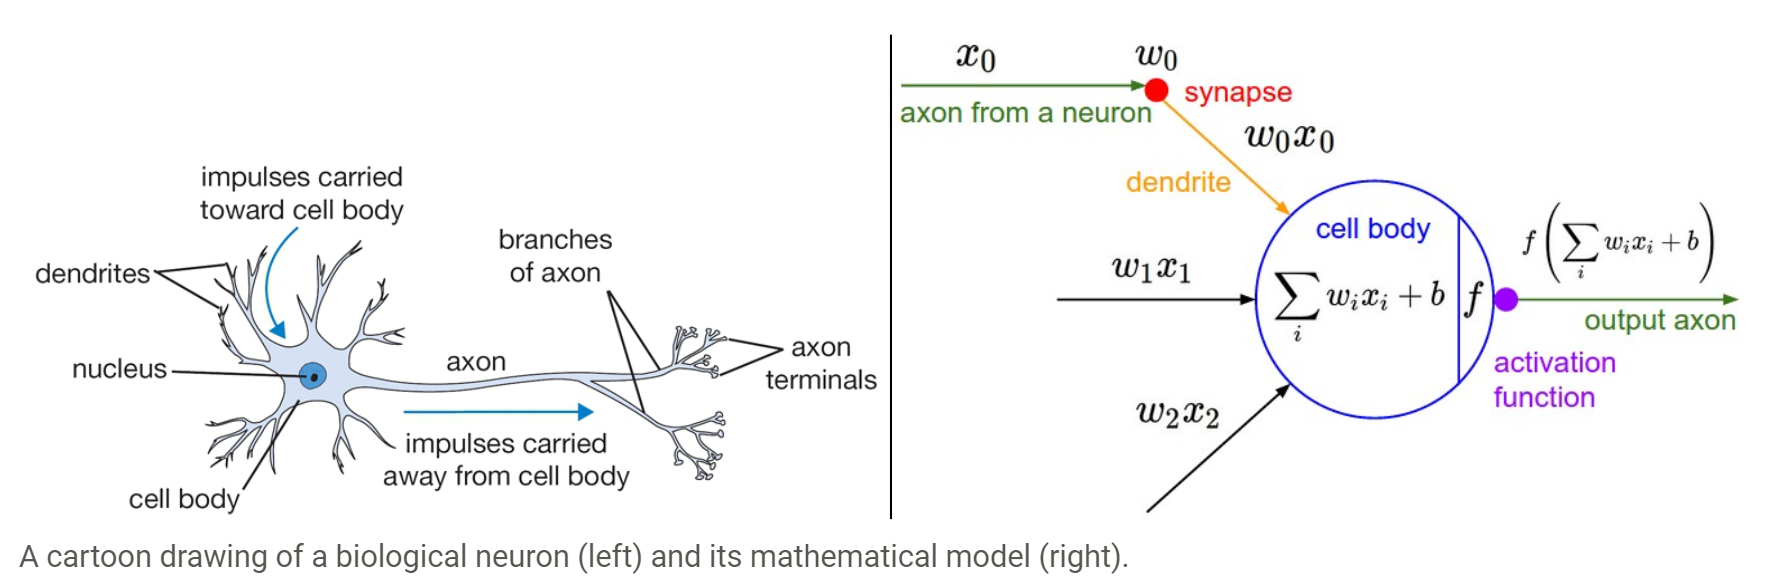
\includegraphics[width=0.9\linewidth]{fig/neuron_model.png}
\caption{\href{http://cs231n.github.io/neural-networks-1/}{神经元}(neuron)}
\end{figure}

常见的激活函数:
\begin{itemize}
    \item Sigmoid:$g(x)=\frac{1}{1+\ee^{-x}}$
    \item Tanh:$g(x)=\tanh(x)=\frac{\ee^{x}-\ee^{-x}}{\ee^{x}+\ee^{-x}}$
    \item ReLU:$g(x)=\max(0,x)$
\end{itemize}
之所以要采用非线性激活函数,是因为它可以使神经网络也变成非线性的,进而捕获到更加复杂的特征。

\begin{figure}[H]
\centering
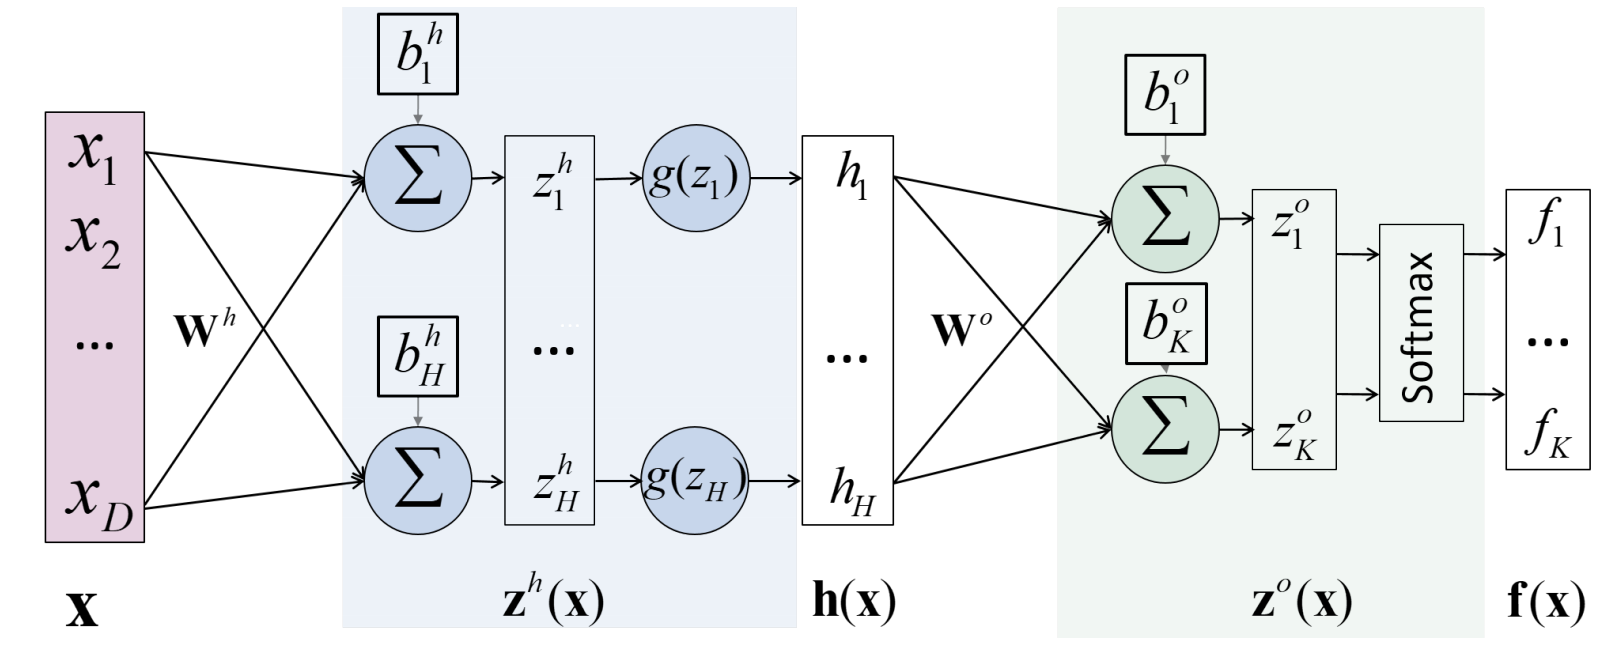
\includegraphics[width=0.8\linewidth]{fig/mlp.png}
\caption{多层神经网络(MLP)}
\end{figure}

但全连接层一个问题在于参数量巨大,当网络变大时计算量将爆炸,故要采用更加好的方法,既能提取出特征,同时计算量也能维持在一个合理的程度,因此就有了\newterm{卷积}(convolution)层。

\subsection{卷积}
$f$为原图,$g$为\newterm{卷积核}(kernel)或\newterm{滤波器}(filter)
\[(f*g)[i,j]=\sum_{m=-M}^M\sum_{n=-N}^Nf[i-m,j-n]g[m,n]\]
即对应元素相乘后相加(但注意卷积与相关操作的不同,\textemph{卷积要先取反})。
卷积在边界时可用0填充(padding)。

上面的公式只是2维卷积,现实我们训练的图片通常采用4维张量表示,即NCHW格式
\[\text{n\_samples}\times \text{n\_channels}\times \text{height}\times \text{width}\]
因此对于每一张多通道的图片,卷积核也应表示为3维,且确保卷积核通道数与图片的通道数相同,这样就可以在3维空间做卷积,但出来的图片只剩1个通道了。
故可以采用\textemph{$k$个权重不同}的卷积核\textemph{分别}对图片做卷积,那么就可以提取到$k$种不同的特征,出来的特征图(feature map)也会有$k$个通道。
% https://m2dsupsdlclass.github.io/lectures-labs/

在具体实施中,卷积层也是可训练的,卷积核的权重和偏置就可以通过网络学习得到。

卷积具有以下三个特征:
\begin{itemize}
    \item \textbf{稀疏交互}(sparse interactions):卷积层不像全连接层,是对整个图像进行权重计算,它只选择与卷积层交叠的部分进行计算。
    参数少了,自然计算量也少了。
    \item \textbf{参数共享}(parameter sharing):由于卷积核是滑过整个图片进行计算,因此对于卷积核的参数,都是被\textemph{多次}运用在不同位置的;而传统的全连接层的参数在图片的每一个位置只会被使用\textemph{一次},因此捕获细节特征的能力也会相对弱一些。
    \item \textbf{平移等变}(equivariant representation):哪怕图片进行一定的平移变换,卷积依然有办法将对应特征提取出来。
\end{itemize}

\bigskip
\begin{tcolorbox}
在图卷积神经网络(GCN)\cite{kipf:gcn_2017}中的卷积也是类似的道理,在一层中的所有图结点采用\textemph{相同}的神经网络进行聚集(aggregate)和更新(update)计算,这样子可以确保神经网络的参数共享,从而关注到图中的局部特征。
\end{tcolorbox}

\subsection{池化}
普通的小卷积只能捕获到低层的特征,想要获得高层的语义特征则卷积核应该有更大的\newterm{感受野}(receptive field),但大卷积又会使图片的细节部分被忽略。
为解决这两者之间的矛盾,可以在\textemph{缩小后的特征图做高层次的卷积}。
那么问题就变成了怎么缩小特征图,常见有两种方法:
\begin{itemize}
    \item 改变步长(stride)
    \item \newterm{池化}(pooling)/\newterm{降采样}(subsampling):对卷积核覆盖的范围取最值或平均
\end{itemize}

池化可以使得表示对于输入的微小变换保持近似不变(invariant),这也是好理解的,因为池化考虑的是一片区域的整体特征,对于取最值或是取平均来说,当局部区域一并改变时,池化后的结果确实不会有太多变化。

\bigskip
\begin{tcolorbox}
看到这好像也就能明白经典的LeNet为什么这么设计了。
先做卷积是为了提取图片中的小的/低层细节特征,然后做激活使得网络非线性,接着做池化,则是将图片进行缩放,方便后续的卷积提取出更大/更高层的语义特征。
\begin{figure}[H]
\centering
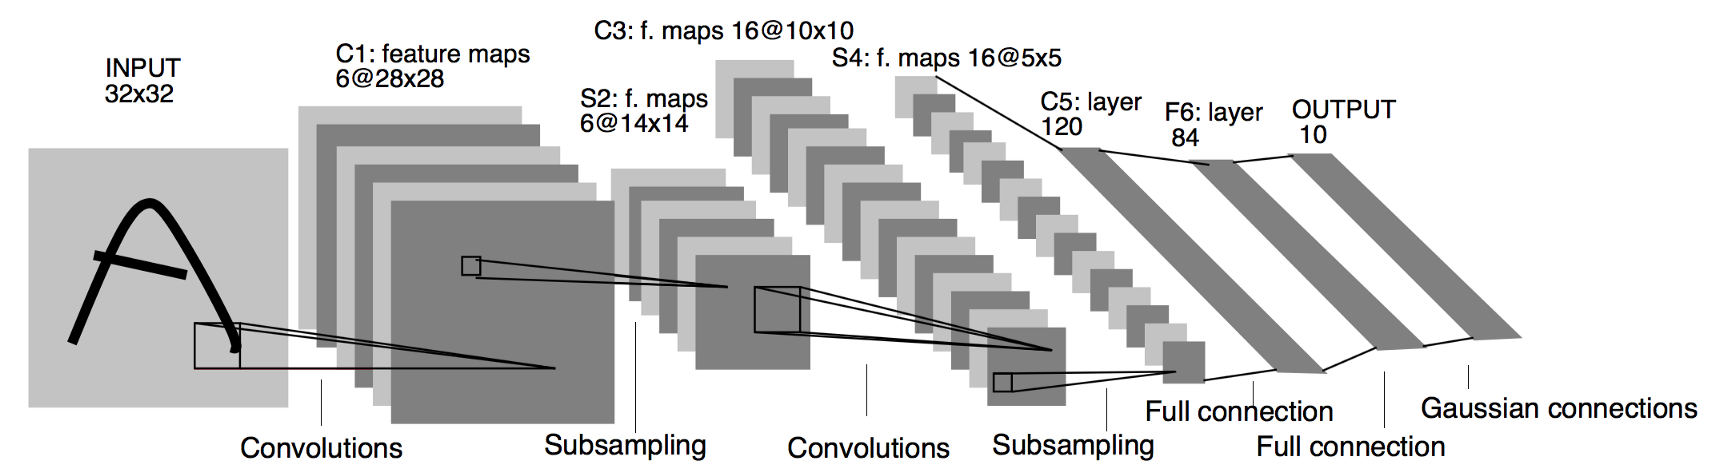
\includegraphics[width=\linewidth]{fig/lenet.png}
\caption{LeNet5}
\end{figure}
\end{tcolorbox}
% !TEX root = main.tex

\section{优化} % ch8, ch7
为了方便叙述,这里采用\href{http://cs229.stanford.edu/notes2019fall/cs229-notes-deep_learning.pdf}{Stanford CS229}的记号,矩阵微积分的推导主要参考:
\begin{itemize}
    \item Andrew Ng, Kian Katanforoosh, Anand Avati, \emph{Stanford CS 229 Lecture Notes: Deep Learning}, \url{http://cs229.stanford.edu/notes2019fall/cs229-notes-deep_learning.pdf}
    \item Andrew Ng, Kian Katanforoosh, \emph{Stanford CS 229 Lecture Notes: Backpropagation}, \url{http://cs229.stanford.edu/notes/cs229-notes-backprop.pdf}
    \item Kaare Brandt Petersen, Michael Syskind Pedersen, \emph{Matrix Cookbook}, \url{https://www.math.uwaterloo.ca/~hwolkowi/matrixcookbook.pdf}
    \item 矩阵求导术 - 长躯鬼侠的文章 - 知乎,\url{https://zhuanlan.zhihu.com/p/24709748}
    \item Daiwk,机器学习中的矩阵、向量求导,\url{https://daiwk.github.io/assets/matrix+vector+derivatives+for+machine+learning.pdf}
\end{itemize}

\subsection{反向传播算法}
设输入特征为$x_1,x_2,\ldots$,即输入层。
$\smp{x}{i}$代表第$i$个训练样本,$\layer{z_j}{l}$代表第$l$层第$j$个神经元的输出,$\layer{a_j}{l}$代表激活后的输出,有
\[\begin{array}{rlrl}
x_1 &= \layer{a_1}{0} & & \\
x_2 &= \layer{a_2}{0} & & \\
\layer{z_1}{1}&=\layer{W_1}{1}^\T\vx+\layer{b_1}{1} &
\layer{a_1}{1}&=g(\layer{z_1}{1})\\
\layer{z_1}{2}&=\layer{W_1}{2}^\T\layer{\va}{1}+\layer{b_1}{2} &
\layer{a_1}{2}&=g(\layer{z_1}{2})
\end{array}\]
其中$W$是参数矩阵,$W_1$代表其中的第1行,激活后的输出为
\[\layer{\va}{1}=\bmat{
    \layer{a_1}{1}\\
    \layer{a_2}{1}\\
    \vdots
}\]

用矩阵的形式写,有
\[\underbrace{
\begin{bmatrix}
    \layer{z_1}{1}\\
    \layer{z_2}{1}\\
    \vdots\\
    \layer{z_m}{1}
\end{bmatrix}}_{\layer{\vz}{1}\in\rr^{m\times 1}}
=\underbrace{
\begin{bmatrix}
    \text{---} & \layer{W_1}{1}^\T & \text{---}\\
    & \vdots & \\
    & \vdots & \\
    \text{---} & \layer{W_m}{1}^\T & \text{---}
\end{bmatrix}}_{\layer{W}{1}\in\rr^{m\times n}}
\underbrace{
\begin{bmatrix}
    x_1\\
    \vdots\\
    x_n
\end{bmatrix}
}_{\vx\in\rr^{n\times 1}}
+\underbrace{
\begin{bmatrix}
    \layer{b_1}{1}\\
    \layer{b_2}{1}\\
    \vdots\\
    \layer{b_m}{1}
\end{bmatrix}
}_{\layer{\vb}{1}\in\rr^{m\times 1}}\]

因此有三层神经网络(单隐含层)的前向传播
\[\begin{aligned}
    \layer{\vz}{1} &= \layer{W}{1}\smp{\vx}{i} + \layer{\vb}{1}\\
    \layer{\va}{1} &= h(\layer{\vz}{1})\\
    \layer{\vz}{2} &= \layer{W}{2}\layer{\va}{1} + \layer{\vb}{2}\\
    \hat{\vy}^{(i)} &=\layer{\va}{2} = g(\layer{\vz}{2})
\end{aligned}\]
其中真实结果$\vy^{(i)}$为独热码(one-hot encoding)。

考虑损失函数(loss)为交叉熵
\[\mL(\hat{\vy},\vy)=-\vy^\T\ln\hat{\vy}^{(i)}\]
且激活函数$h(\cdot)$为sigmoid函数,$g(\cdot)$为softmax函数。

接下来推导反向传播(backpropagation, BP)算法,利用链式法则求导数。
比如想得到隐含层的权重,则计算
\[\pd{\mL}{\layer{W}{2}}=\pd{\mL}{\layer{\va}{2}}\pd{\layer{\va}{2}}{\layer{\vz}{2}}\pd{\layer{\vz}{2}}{\layer{W}{2}}\]
注意上式并非良定,其中涉及到实值函数对向量求导,也涉及到向量对向量求导(雅可比矩阵),还有向量对矩阵求导。
\[\begin{aligned}
\pd{\mL}{\layer{\va}{2}}
&=\pd{}{\layer{\va}{2}}(-\vy^\T\ln\hat{\va}^{[2]}) \qquad\mbox{实数对向量求导}\\
&=-\frac{\vy}{\layer{\va}{2}} \qquad\mbox{逐元素相除}
\end{aligned}\]

设$\vu=\exp(\layer{\vz}{2})$为逐元素指数,分两步计算
\[\begin{aligned}
\pd{\layer{\va}{2}}{\vu}
&=\pd{}{\vu}\softmax(\layer{\vz}{2})\\
&=\pd{}{\vu}\frac{\exp(\layer{\vz}{2})}{\vone^\T\exp(\layer{\vz}{2})}\\
&=\pd{}{\vu}\frac{\vu}{\vone^\T\vu}\\
&=\vu\pd{(1/\vone^\T\vu)}{\vu^\T}+\frac{1}{\vone^\T\vu}\pd{\vu}{\vu} \qquad\mbox{乘法法则}\\
&=-\frac{1}{(\vone^\T\vu)^2}\vu\vone^\T+\frac{1}{\vone^\T\vu}I\\
\pd{\vu}{\layer{\vz}{2}}
&=\pd{\exp(\layer{\vz}{2})}{\layer{\vz}{2}}\\
&=\diag(\exp(\layer{\vz}{2}))\\
&=\diag(\vu)
\end{aligned}\]

由雅可比矩阵的链式法则
\[\begin{aligned}
\pd{\layer{\va}{2}}{\layer{\vz}{2}}
&=\pd{\layer{\va}{2}}{\vu}\pd{\vu}{\layer{\vz}{2}}\\
&=\lrp{-\frac{1}{(\vone^\T\vu)^2}\vu\vone^\T+\frac{1}{\vone^\T\vu}I}\diag(\vu)\\
&=-\frac{1}{(\vone^\T\vu)^2}\vu\vu^\T+\frac{1}{\vone^\T\vu}\diag(\vu)\\
&=-\frac{\vu}{\vone^\T\vu}\lrp{\frac{\vu}{\vone^\T\vu}}^\T+\frac{1}{\vone^\T\vu}\diag(\vu)\\
&=-\layer{\va}{2}\layer{\va}{2}^\T+\diag(\layer{\va}{2})
\end{aligned}\]

进而
\[\begin{aligned}
\pd{\mL}{\layer{\vz}{2}}
&:=\layer{\delta}{2} \qquad\mbox{损失函数对未激活前$\vz$的导数}\\
&=\lrp{\pd{\layer{\va}{2}}{\layer{\vz}{2}}}^\T\pd{\mL}{\layer{\va}{2}}\\
&=-\lrp{-\layer{\va}{2}\layer{\va}{2}^\T+\diag(\layer{\va}{2})}^\T\lrp{\frac{\vy}{\layer{\va}{2}}}\\
&=\layer{\va}{2}\lrp{\layer{\va}{2}^\T\frac{\vy}{\layer{\va}{2}}}-\diag(\layer{\va}{2})\lrp{\frac{\vy}{\layer{\va}{2}}}\\
&=\layer{\va}{2}\vone^\T\vy-\vy\\
&=\layer{\va}{2}-\vy \qquad\mbox{独热码满足$\vone^\T\vy=1$}
\end{aligned}\]

之后可计算
\[\begin{array}{lll}
\pd{\mL}{\layer{W}{2}}&=\pd{\mL}{\layer{\vz}{2}}\pd{\layer{\vz}{2}}{\layer{W}{2}}
&=\layer{\delta}{2}\layer{\va}{1}^\T \qquad\mbox{线性变换求导法则}\\
\pd{\mL}{\layer{b}{2}}&=\pd{\mL}{\layer{\vz}{2}}\pd{\layer{\vz}{2}}{\layer{b}{2}}
&=\layer{\delta}{2}
\end{array}\]

再往前推一层
\[\begin{aligned}
\pd{\mL}{\layer{\va}{1}}
&=\layer{W}{2}^\T\layer{\delta}{2}\\
\pd{\mL}{\layer{\vz}{1}}
&:=\layer{\delta}{1}\\
&=\pd{\mL}{\layer{\va}{1}}\pd{\layer{\va}{1}}{\layer{\vz}{1}}\\
&=\pd{\mL}{\layer{\va}{1}}\odot h'(\layer{\vz}{1})\\
&=\lrp{\layer{W}{2}^\T\layer{\delta}{2}}\odot h(\layer{\vz}{1})\odot (\vone-h(\layer{\vz}{1}))\\
\pd{\mL}{\layer{W}{1}}&=\layer{\delta}{1}\vx^\T\\
\pd{\mL}{\layer{\vb}{1}}&=\layer{\delta}{1}\\
\pd{\mL}{\vx}&=\layer{W}{1}^\T\layer{\delta}{1}
\end{aligned}\]

总结来说,对于$l=N-1,N-2,\ldots,1$层,设\textcolor{red}{
\[\layer{\delta}{l}=\lrp{\layer{W}{l+1}^\T\layer{\delta}{l+1}}\odot h'(\layer{\vz}{l})\]
}
则有权重和偏置的梯度\textcolor{red}{
\[\begin{aligned}
\nabla_{\layer{W}{l}}\mL(W,b)&=\layer{\delta}{l}\layer{\va}{l-1}^\T\\
\nabla_{\layer{b}{l}}\mL(W,b)&=\layer{\delta}{l}
\end{aligned}\]
}

\subsection{梯度下降}
\begin{itemize}
    \item 批梯度下降
    \[\vtheta_{t+1}=\vtheta_t-\frac{\eta}{N}\sum_{n=1}^N\nabla\mL(\vy_n,\vf(\vx_n;\vtheta_t))\]
    \item 随机梯度下降(SGD)
    \[\vtheta_{t+1}=\vtheta_t-\eta\nabla\mL(\vy_n,\vf(\vx_n;\vtheta_t))\]
    \item 子批(minibatch)梯度下降
    \[\vtheta_{t+1}=\vtheta_t-\frac{\eta}{|S|}\sum_{(\vx_n,\vy_n)\in S}\nabla\mL(\vy_n,\vf(\vx_n;\vtheta_t))\]
\end{itemize}

添加动量(momentum)项,使得梯度下降可以保持原来的方向,以减少震荡
\[\begin{cases}
    \vnu_{t+1}=\textcolor{red}{\gamma\vnu_t}+\eta\nabla\mL(\vtheta_t)\\
    \vtheta_{t+1}=\vtheta_t-\vnu_{t+1}
\end{cases}\]
通常$\gamma$取$0.9$。

\subsection{过拟合}

\newpage
\bibliographystyle{unsrt}
\bibliography{dl}

\end{document}